%
% ---------------------------------------------------------------------------------------
% VaLOR T2K numu disappearance analysis, Run1+2+3
% ---------------------------------------------------------------------------------------
%

\documentclass[final]{elsarticle}

\usepackage[margin=2.50cm]{geometry}  % tweak margins
%\usepackage{draftcopy}                % uncomment to print a "DRAFT-COPY" in background
\usepackage{graphicx}                 % if you want to include PostScript figures
\usepackage[figuresright]{rotating}   % if you have landscape tables
\usepackage{multirow}                 % fancy tables
\usepackage[toc,page]{appendix}       % appendix
\usepackage{lineno}                   % for printing the line numbers
\usepackage{natbib}                   % for building bibliography with \cite{}
\usepackage{setspace}
\usepackage{times}
\usepackage{afterpage}
\usepackage{float}
\usepackage{subfigure}
\usepackage{color} 
\usepackage{rotate}                   % rotate text in tables
\usepackage{amsfonts}                 % extra symbols
%%%% This must be the last usepackage
\usepackage[breaklinks=true]{hyperref}% allow use of url; ref & cite are hyperlinks

% use to fix date
% \def \today { February 1st, 2009 }
% put your own definitions here:
\newcommand{\ck}{$\checkmark$}
\newcommand{\ttbs}{\char'134}
%\newcommand{\AmS}{{\protect\the\textfont2
%  A\kern-.1667em\lower.5ex\hbox{M}\kern-.125emS}}
% add words to TeX's hyphenation exception list
%\hyphenation{author another created financial paper re-commend-ed Post-Script}

% By default, LaTeX doesn't like to fill more than 0.7 of a text page with tables and graphics, 
% nor does it like too many figures per page. This behaviour can be changed:
\renewcommand\floatpagefraction{.9}
\renewcommand\topfraction{.9}
\renewcommand\bottomfraction{.9}
\renewcommand\textfraction{.1}   
\setcounter{totalnumber}{50}
\setcounter{topnumber}{50}
\setcounter{bottomnumber}{50}

\linenumbers
\bibliographystyle{elsart-num}

\begin{document}

% Title, authors, abstract and table of contents
%
% Front matter
%

\begin{frontmatter}

\title{
  Revision history and replies to comments on T2K-TN-155\\
  {\em(T2K 6.3933$\times10^{20}$-POT 3-Flavour Muon-Neutrino Disappearance Analysis)}
}

\vspace*{0.7cm}

\author[RAL]     {Costas Andreopoulos}
\author[RAL,OXF] {Thomas Dealtry}
\author[IFIC]    {Lorena Escudero S\'anchez}
\author[LANCS]   {Nick Grant}
\author[RAL,OXF] {and Alfons Weber}

\address[RAL]{Particle Physics Dept., Rutherford Appleton Laboratory, STFC \\
              Harwell Oxford Campus\\
              Oxfordshire OX11 0QX, UK}

\address[OXF]{Subdepartment of Particle Physics, University of Oxford \\
              Denys Wilkinson Building, Keble Road\\
              Oxfordshire OX1 3RH, UK}

\address[IFIC]{Instituto de Fisica Corpuscular\\
              CSIC and University of Valencia\\
              Valencia, Spain}

\address[LANCS]{Physics Dept., Lancaster University \\
              Lancaster, LA1 4YB, UK}

%
% Abstract
%

\begin{abstract}

The results of the {\em VaLOR} (Valencia-Lancaster-Oxford-Rutherford) 
3-flavour $\nu_{\mu}$-disappearance analysis on the combined Run1+2+3+4a dataset 
were reported in T2K-TN-155v1.
All comments received from the analysis review committee and the collaboration
are addressed, in detail whenever required, in this addendum.
Revisions of T2K-TN-155 made as a response to these comments 
are also summarized here.

\end{abstract}

\end{frontmatter}

%\clearpage

\tableofcontents

\clearpage





% Main body
\section{Replies to comments (on version 1 of T2K-TN-155) received from the review committee}

{\color{red}
Please note that all section, figure, table, equation, footnote and citation 
numbers mentioned in this section refer to T2K-TN-155v1. 
The corresponding numbers in later versions of the note may be different.
}
\subsection{
  Replies to comments received from Scott Oser - Aug 09, 2013 }

\begin{enumerate}

  % ........................................................................................................
  \vspace{5 mm}
\item
  {\em
    The document contains 1D parameter limits on $\Delta m^2$ and $\sin^2(\theta_{23})$, based on a profile likelihood method.
    This is good, but I think it's very important that proper 1D Feldman-Cousins confidence intervals also be presented.
    Without these the analysis is not complete.  I have spoken with Tom about this in the past, and I think we agreed that
    this could be done by throwing $\Delta m^2$ values for the toy simulations according to T2K's marginalized likelihood for
    $\Delta m^2$. Perhaps this work is already in progress and will be given to us soon, but I don't think this is optional.
    We had a lot of confusion and delay inside the collaboration because these were not available for the Run 1+2+3 result,
    and we need to make sure we do it right this time.
  }\\
  \\
  We agree that 1D FC is important to include. It was not included in v1 due to time pressures.
  A description of the proposed method is available in v2.
  The first result using this method will be in v3, when we have the
  final inputs to the analysis.
  

  % ........................................................................................................
  \vspace{5 mm}
\item
  {\em
    There are many, many differences between the BANFF input values listed in the table on p. 13 and the values given
    in the latest BANFF TN-166, which worries me.  Most numbers differ in the 2nd or 3rd decimal point, and some differ
    considerably.  The most glaring example is the resonance-production axial-mass scaling factor.  TN-166 Table 11 says
    this fits to 0.963386 GeV, which if I divide by its nominal value of 1.41 GeV gives a scale factor of 0.683, which is
    very different from the value of 0.796 listed here.  The CC1pi normalizations are also noticeably different from TN-166 values.  
  }\\
  \\
  TN155 uses \verb+postfit_banff_2013_disappearance_v4.root+. Versions 1 \& 2 of TN166 refers to an older
  version of the BANFF fit. TN166v3 is an update with the v4 fit results.

  % ........................................................................................................
  \vspace{5 mm}
\item
  {\em
    p. 16, footnote 2:\\
    You have a very large number of bins in your 2D MC templates.  This makes me worry if you have enough MC statistics.
    Almost certainly you need to include a systematic uncertainty to represent the contribution from finite MC statistics,
    but I see no mention of that in this tech note or in TN-141, unless I missed one.
    This may not be a small effect when you have so many bins, so I think it needs to be addressed.
  }\\
  \\
  In the 13a SKMC, there are 426043 1-ring $\mu$-like events:
  \begin{itemize}
  \item 275649 $\nu_\mu$;
  \item 132423 $\bar{\nu_\mu}$.
  \item 9133 $\nu_e$;
  \item 4871 $\bar{\nu_e}$;
  \item 3967 oscillated $\nu_e$.
  \end{itemize}
  We then split these up into 32 interaction mode bins\footnote{
    We actually reuse the CC events of the $\nu_\mu$ sample to fill
    the four $\nu_e \rightarrow \nu_\mu$ templates.
    \\We don't use the NC events of the oscillated $\nu_e$ sample.
  }, 73 $E_{reco}$ bins \& 84 $E_{true}$ bins 
  (196224 total bins).

  The method used to study the SKMC statistical error is, for each of the 73 $E_{reco}$ bins:
  \begin{itemize}
  \item Sum the mean square of 32 modes \& 84 $E_{true}$ bins that make
    up the $E_{reco}$ bin 10000 times, using Poisson throws
  \item Calculate the RMS by dividing the sum mean square by sqrt(10000)
  \item Error = RMS / nominal
    \begin{itemize}
    \item No POT scaling, flux weights, systematics, or oscillations applied
      \\(It's the number of events from the MC in the bin)
    \end{itemize}
  \item Compare with:
    \begin{itemize}
    \item The error from 100000 toys in which all systematics are thrown
    \item The Run 1-4 statistical error
    \end{itemize}
  \end{itemize}
  The fractional error is shown in Fig.\ \ref{fig:mc_stat_err_spectrum} of this document, where the statistical error has been calculated for 3 situations:
  \begin{itemize}
  \item 1 $E_{true}$ bin * 1 mode is the MC stat error calculated on the total $E_{reco}$ spectrum (73 bin total);
  \item 84 $E_{true}$ bin * 32 mode is the MC stat error calculated on the individual modes' $E_{true}$-$E_{reco}$ templates (196224 bin total);
  \item 84 $E_{true}$ bin * 32 mode is the MC stat error calculated on the individual modes' $E_{true}$-$E_{reco}$ templates (196224 bin total) + double MC statistics.
  \end{itemize}
  While it will not produce an large effect on the total systematic error budget,
  it does have a larger effect than some of the systematic parameters we consider
  (compare with Figs.\ 1-45 of the supplementary material for TN155).

  The ratio of MC statistical error to the total systematic error is shown in Fig.\ \ref{fig:mc_stat_err_ratio}
  of this document.
  The figure shows that in the oscillation dip region, the MC statistical error is $\approx$8\% of the total
  systematic error.
  The MC statistical error does however increase at higher energies.

  The ratio of both MC statistical error and systematic error, to the Run 1-4 statistical error
  is shown in Fig.\ \ref{fig:mc_stat_err_ratio_stat} of this document.
  The figure shows that the Run 1-4 statistical error dominates the MC statistical error
  at all energies.

  We feel that the size of the MC statistical error is small enough in the important
  part of the spectrum (oscillation dip region), compared 
  with the total systematic error, to be neglected in this analysis.

  In future analyses, we suggest that a higher POT of SKMC be generated.
  Generating an independent $\nu_e \rightarrow \nu_\mu$ sample is also useful.
  Studies were done in Run 1-3 on the $E_{true}$ binning, which found
  that the 84-bin scheme is required to be able to apply accurate oscillation probabilities.
  See Appendix I.1 of T2K-TN-141 for details (a 70-bin scheme was also tried, and was found to have
  too large a deviation from the 780-bin scheme).
  Similary, we should be careful to reduce the $E_{reco}$ binning, since the
  shape information in the fit is encoded here. The 78-bin scheme we use
  does contain enough information compared with the 50 MeV (600-bin) scheme
  used in Run 1+2, as can be seen in Appendix I.2 of T2K-TN-141.
  Some further optimisation may be possible.
  
  \begin{figure*}[htb]
    \center
    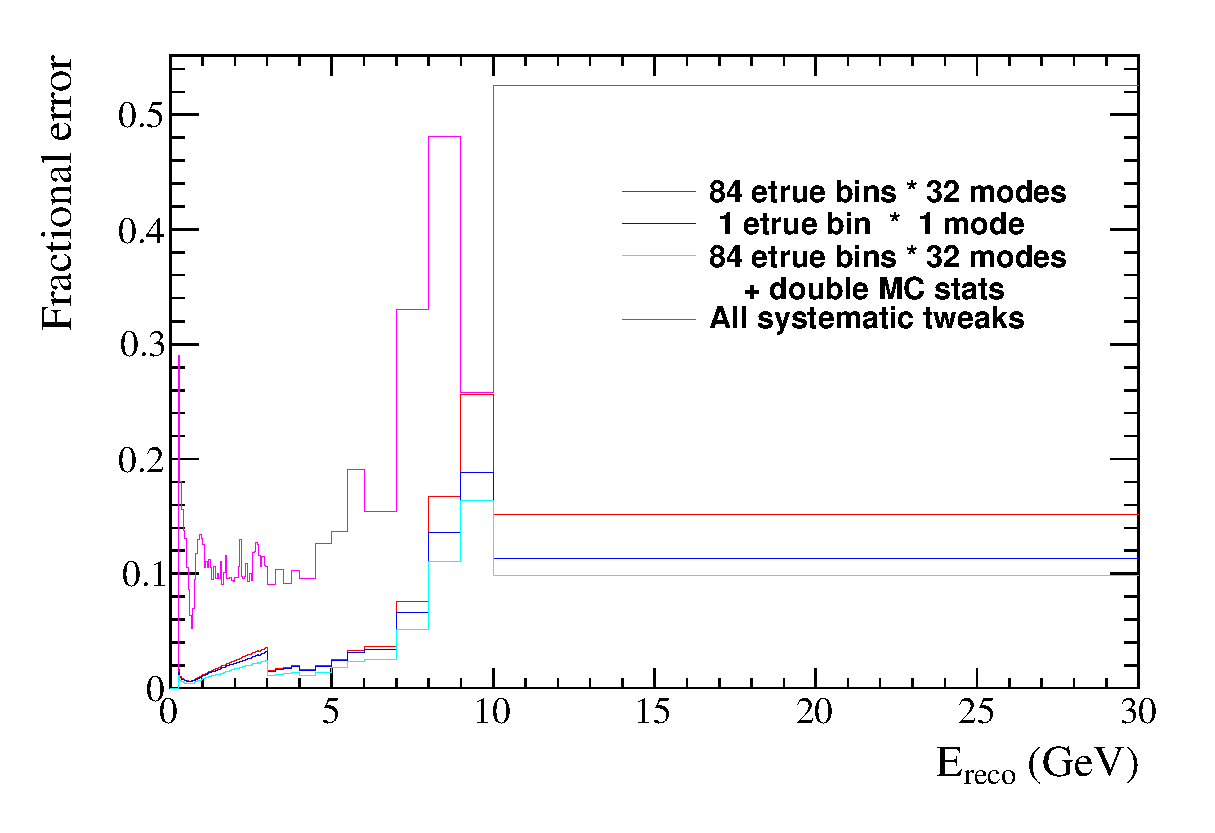
\includegraphics[width=30pc]{./images/mcstaterr_spectrum}
    \caption {
      Fractional error on $N_{SK}$ for three types of statistical error,
      and the total systematic error.
      No oscillations have been applied.
    }
    \label{fig:mc_stat_err_spectrum}
  \end{figure*}

  \begin{figure*}[htb]
    \center
    \begin{minipage}[htb]{0.45\linewidth}
      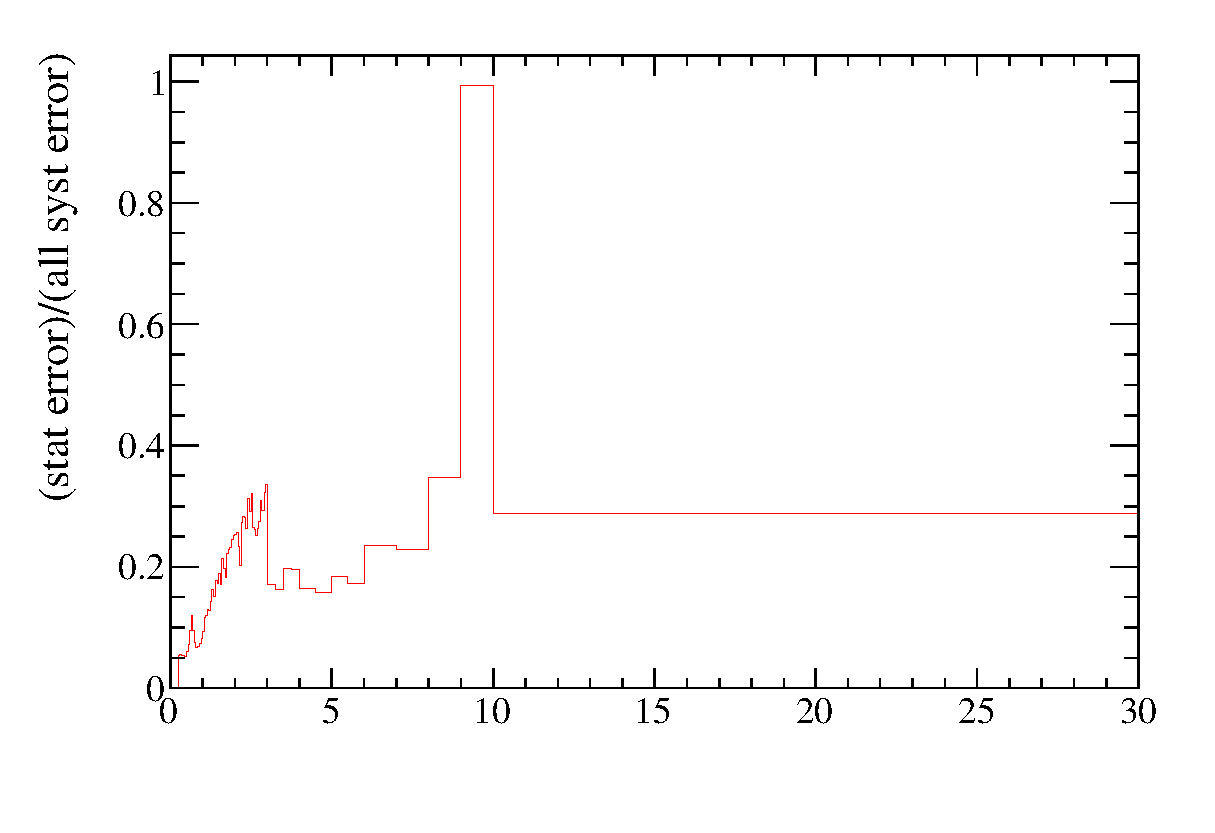
\includegraphics[width=20pc]{./images/mcstaterr_ratio}
      \caption {
        Ratio of MC statistical error to total systematic error.
        No oscillations have been applied.
      }
      \label{fig:mc_stat_err_ratio}    
    \end{minipage}
    \hspace{0.06\linewidth}
    \begin{minipage}[htb]{0.45\linewidth}
      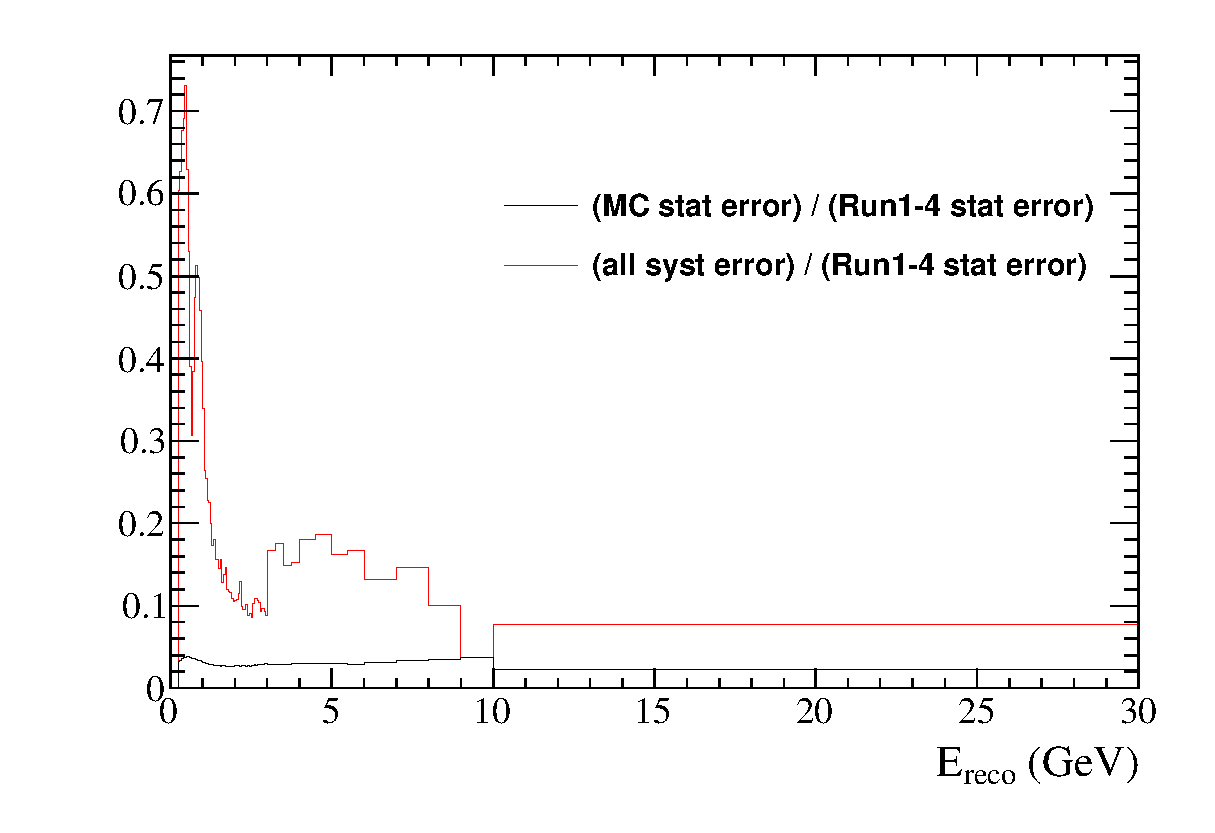
\includegraphics[width=20pc]{./images/mcstaterr_ratio_stat}
      \caption {
        Ratio of MC statistical error and total systematic error
        to Run 1-4 statistical error.
        No oscillations have been applied.
      }
      \label{fig:mc_stat_err_ratio_stat}    
    \end{minipage}
  \end{figure*}

  
  % ........................................................................................................
  \vspace{5 mm}
\item
  {\em
    Figs 59-61:\\
    The 90\% CL horizontal line on these plots seems to be drawn at 2.3, rather than the correct value of 2.7.
    This makes me concerned that you have miscalculated the 90\% 1D confidence intervals in Fig 61.
    Please check this, and state explicitly what $\Delta(\chi^2)$ values were used for the 68\% and 90\% CL limits in Fig 61.
    (Of course I've already stated that I think the FC equivalents are a mandatory addition.)
  }\\
  \\
  You are correct that the incorrect value was used. The plots \& 1D limits have been updated.
  1D limits are calculated using $\Delta \chi^2 =$ 1.00(2.71) for 68\%(90\%).
  2D contours are calculated using $\Delta \chi^2 =$ 2.30(4.61) for 68\%(90\%).
  A footnote has been added to section 7.4 with these values.

  % ........................................................................................................
  \vspace{5 mm}
\item
  {\em
    Given that we haven't had any new data in months, and won't have any, why shouldn't we immediately extend
    this analysis to include ALL Run 4 SK data?  I wouldn't propose to update the ND280 inputs,
    but it really shouldn't be much work to add in the late April-early May 2013 data, should it?
    The beam systematics for that period will almost certainly be identical to that for the rest of Run 4,
    and although the beam inputs to the BANFF fit will have to be adjusted for a slightly different POT weighting,
    this ought to be very fast.  We're going to need to do this anyway, so why not now?
  }\\
  \\
  The decision to use only Run 1-4a data for the first version of
  the 2013 $\nu_\mu$ disappearance analysis was taken by the collaboration.
  The collaboration also agreed to move to the full Run 1-4 dataset for the
  September collaboration meeting.
  Therefore v3 of the note will include all data recorded.

  % ........................................................................................................
  \vspace{5 mm}
\item
  {\em
    Line 435-436:\\
    I find it a little strange that you are throwing random values for $\delta_{CP}$ in the fake data sets
    but are not allowing $\delta_{CP}$ to float in the fit.  It seems a little inconsistent to do one but not the other.
    Can you please justify this choice?
  }\\
  \\
  The constant-$\Delta\chi^2$ normal hierarchy contours for
  $\delta_{CP} = -\pi/2$, 0, $+\pi/2$, $+\pi$
  is shown
  in Fig.\ \ref{fig:constdchisqcontours_changedcp} of this document.
  It can be seen that changing $\delta_{CP}$ has almost no effect on the contour.
  For this reason, and due to the fact that the typical fit time is increased
  by 10\% by including $\delta_{CP}$, it was decided not to fit for it in v1.

  \begin{figure*}[htb]
    \center
    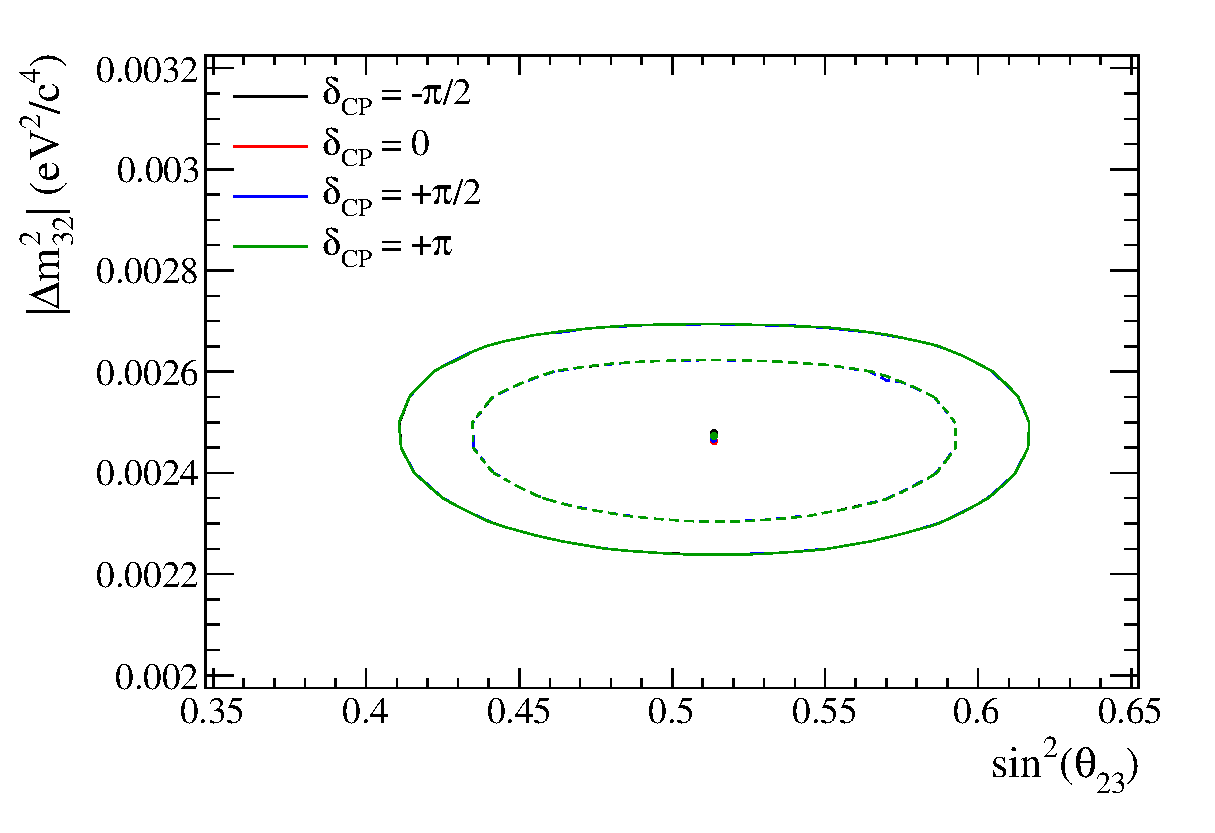
\includegraphics[width=30pc]{./images/contours_run1-4a_nuis3fixdcp_dcp}
    \caption {
      68\% CL and 90\% CL allowed region (including systematics), 
      constructed with the constant-$\Delta\chi^{2}$ method,
      for the fit to the Run 1+2+3+4a dataset,
      for four assumptions of the value of
      $\delta_{CP} = -\pi/2$, 0, $+\pi/2$, $+\pi$.
      The best-fit points are also shown.
      The normal mass hierarchy is assumed.
    }
    \label{fig:constdchisqcontours_changedcp}
  \end{figure*}

  Fitter bias studies have been performed for
  the case where $\delta_{CP}$ is fit for, and compared to the studies
  where $\delta_{CP}$ is set to 0.
  No obvious issues have been found\footnote{
    The pull distribution of $\delta_{CP}$ is irregular,
    due to it having a small effect on the 1-ring $\mu$-like energy spectrum,
    and there being no constraint term, the HESSE assigns
    large errors.
    However this has no effect on the distributions of other parameters.
  }
  to suggest that
  fitting for $\delta_{CP}$ is not possible.
  Therefore in v3 of the note, we will include $\delta_{CP}$ in the fit
  as a free parameter, with no constraint term.

  
  % ........................................................................................................
  \vspace{5 mm}
\item
  {\em
    I have a picky question about the CC1pi normalization (parameter \#21) on p. 13.  The BANFF nominal value (pre-BANFF fit) is 1.15,
    according to TN-166, and you list the fitted value as 1.200 (although TN-166 gives 1.217 instead).  My question
    (besides why 1.200 instead of 1.217) is whether you are interpreting the fitted value as a scale factor relative to 1.15, or
    relative to 1.0?  That is to say, based on the fitted value, do you scale the CC1pi events for this bin by 1.200, or by
    (1.15 x 1.200)?  I don't even know for sure which is right---you may need to ask the BANFF experts.
    Really I just want some reassurance that everyone is interpreting this scale factor consistently.  All(?) of the
    other scale factor parameters have nominal values of 1.0, so this question may not arise for them.
  }\\
  \\
  The discrepancy in values is due to inconsistent BANFF fit versions described in the notes.
  We treat it as (1.00 x 1.200).
  I have confirmed with Mark Hartz that is correct.
  
  % ........................................................................................................
  \vspace{5 mm}
\item
  {\em
    p. 13:\\
    please state explicit the form of the constraint term, if any, for $f_{SF; t, r}$.  I couldn't find it in TN-141 either.
    I'm guessing that you have no constraint term other than bounding the parameter to the region [0,1]?  Please confirm.
  }\\
  \\
  For v1 of the note, there is a constraint term, and it has the same form as any other systematic terms. Namely,
  \begin{equation}
    \frac{f_{bf} - f_{nom}}{\sigma_{nom}^2},
  \end{equation}
  since it is not correlated with any other systematic.
  The boundary of [0,1] is also applied, meaning the penalty runs from [0,1].

  After thinking about this,
  for v3 of the note, we will have no constraint term.
  This is because we throw the parameter uniformly in the range [0,1]
  when generating toy experiments, and so having a constraint which favours
  $f_{SF; t, r} = 0$ is unnatural.

  % TN113v1.2
  % 471 The uncertainty is scaled such that the 1σ uncertainty is set to be the difference
  % 472 between SF and FG, 0 is no difference, and all other values are linearly extrapolated
  % 473 or interpolated (e.g. 2σ is twice the SF/FG difference). While this is nonphysical,
  % 474 it was not obvious how to treat a discrete (on/off) parameter in the 2012a fits. In
  % 475 addition, a smooth parametrization allows us to see where the fit moves this nuisance
  % 476 parameter according to agreement with data. An inherent limitation to the current
  % 477 parametrization is that the SF prediction populates regions of true p − θ where FG
  % 478 does not, and this cannot be treated with reweighting. An example of this can be
  % 479 seen in Figure 64 which shows NuWro SF populates p < 0.3 GeV/c and cos(θ) > 0.3,
  % 480 not present in either FG model; note that the cross section in this region is much
  % 481 smaller than in the primary region.

  % ........................................................................................................
  \vspace{5 mm}
\item
  {\em
    Pull distribution figures:\\
    why is the width of the pull distribution for $f^{SK}_{E;r}$ usually 1.15 instead of the expected 1.0. 
  }\\
  \\
  This is to do with the fact that the effect of the $f^{SK}_{E;r}$ systematic on
  the number of events in a bin is not a smooth function of $f^{SK}_{E;r}$;
  it is continuous, but it's differential is not.
  This is due to the systematic being dependant on the number of events in neighbouring bins,
  and so there is a discontinuity in the differential when moving from positive to negative
  values of $f^{SK}_{E;r}$, and also at large values of $f^{SK}_{E;r}$ when next-to-neighbouring
  bins come into effect.
  Therefore HESSE has a problem evaluating errors for this parameter.
  If we instead use MINOS errors, the distribution is as expected, as shown
  in Fig.\ \ref{fig:skescale_pull} of this document.
  The residual distribution exhibits the correct behaviour.

  \begin{figure*}[htb]
    \center
    \includegraphics[width=25pc]{{./images/fixdcpminos_sys_0.37_pull_1_escale}.eps}
    \caption {
      Pull distribution for $f^{SK}_{E;r}$,
      computed from 5.1k toy MC experiments at 6.3933×1020 POT,
      generated at
      at $\sin^2\theta_{23} = 0.65$ and $|\Delta m^2 | = 2.4\times10^{−3}$ eV$^2$/c$^4$, including
      statistical fluctuations and with randomized systematic parameters.
      MINOS errors are used.
    }
    \label{fig:skescale_pull}
  \end{figure*}

  % ........................................................................................................
  \vspace{5 mm}
\item
  {\em
    Fig 17:\\
    I understand the three peaks in Figs 15 and 19 (true point, mirror point, and point of maximum disappearance).
    But I don't understand Fig 17, where there are also three humps (although two are quite small), even
    though the best-fit point should be the same as the point of maximual disappearance.  Please comment.
  }\\
  \\
  This is still under study.

  % ........................................................................................................
  \vspace{5 mm}
\item
  {\em
    Line 371:\\
    Shouldn't you be citing Ref [22] rather than Ref [15], and referring to CC0pi, CC1pi, and CCother samples rather
    than CCQE and CCnQE?  Doesn't this analysis use the 2013 BANFFv2 fit results and not 2012 BANFF fits?
  }\\
  \\
  Correct, this has been updated.

  % ........................................................................................................
  \vspace{5 mm}
\item
  {\em
    Line 442:\\
    point of clarification: do these 7 parameters include 1 energy scale and 6 detector/FSI efficiency parameters?
  }\\
  \\
  Yes.
  The bullet point list \& Tab.\ 1 headings have been updated.
  
  % ........................................................................................................
  \vspace{5 mm}
\item
  {\em
    Top of p. 13:\\
    again you are citing Ref [15] (old BANFF) rather than [22] (new 2013 BANFF).  Why?  
  }\\
  \\
  This has been corrected.

  % ........................................................................................................
  \vspace{5 mm}
\item
  {\em
    Table 3:\\
    Of course I can't imagine it mattering, but why did you use $\Delta m^2_{21}=7.5\times 10^{-5}$
    instead of the PDG2012 value of $7.58\times 10^{-5}$?
  }\\
  \\
  When choosing values of oscillation parameters, we have used the particle
  listings section of reference 28.

  The value $7.58 \times 10^{-5}$ is shown on p193,
  which is in the review of neutrino mixing, and is the result of a
  3-flavour fit, incorporating neutrino oscillation data (but not Daya Bay \& RENO).
  
  The value $7.50 \times 10^{-5}$ is shown on p642,
  which is the particle listings, and is the result of a 3-flavour fit
  on KAMLAND + solar data.

  % ........................................................................................................
  \vspace{5 mm}
\item
  {\em
    Table 7:\\
    are the values in this table in percent?  If so, please state that in the caption.
  }\\
  \\
  Yes, this has been corrected.

  % ........................................................................................................
  \vspace{5 mm}
\item
  {\em
    Pull distribution figures:\\
    several figures have fitted means of 1.0 and sigmas of 0.  This can't be right.  I'm guessing these are failed fits---can you please fix them?
  }\\
  \\
  There are 4 fits that had a fitted sigma of 1, with an error on this value of 0.0 according to the plots.
  All 4 fits were fine (no failed fits) it was just the way ROOT was reporting the error in the stat box
  (it appears that ROOT rounds \& kills trailing zeros in the parameter value, then quotes errors to this significance).
  The plots have been updated with more significant figures in the fit stat box.
  
  % ........................................................................................................
  \vspace{5 mm}
\item
  {\em
    Fig 49, and many other figures:\\
    The legends printed on this plot, and those like them, are too small to be acceptable for publication in Phys. Rev.
    If these are to become official plots, please remake them with larger, more legible legends.
  }\\
  \\
  We have increased the legend size of some plots in v2 of the note,
  but have not done them all, since for some plots this was the only comment.
  When we release v3, with the results from the fixed SuperK detector error matrix,
  we will update the legends in the rest of the plots.
  
  % ........................................................................................................
  \vspace{5 mm}
\item
  {\em
    Figs 55 \& 56 captions:\\
    You mean Run 1+2+3+4a, not Run 1+2+3
  }\\
  \\
  This has been corrected.

  % ........................................................................................................
  \vspace{5 mm}
\item
  {\em
    Line 734:\\
    How was the marginalization by octant done?  Did you average the contours, or did you simply take the larger of the two contours?
  }\\
  \\
  From D. Karlen's comments on the Run 1-3 PRL, we realise that the wrong terminology was originally used.
  The method is, in fact, profiling.
  
  For every point in $\sin^2(2\theta_{23})$ there are 2 points in $\sin^2\theta_{23}$ for which the $\Delta \chi^2$
  and $\Delta\chi^2_{crit}$ are known.
  The $\sin^2\theta_{23}$ point with the lowest $\Delta\chi^2 - \Delta\chi^2_{crit}$ is chosen.
  The $\sin^2(2\theta_{23})$ contour created will be similar to the second octant contour
  if an octant preference is made.
  Fig.\ \ref{fig:contours_sinsq2theta_method} of this document shows that in this case, the
  profiled and second octant contours are identical.  

  \begin{figure*}[htb]
    \center
    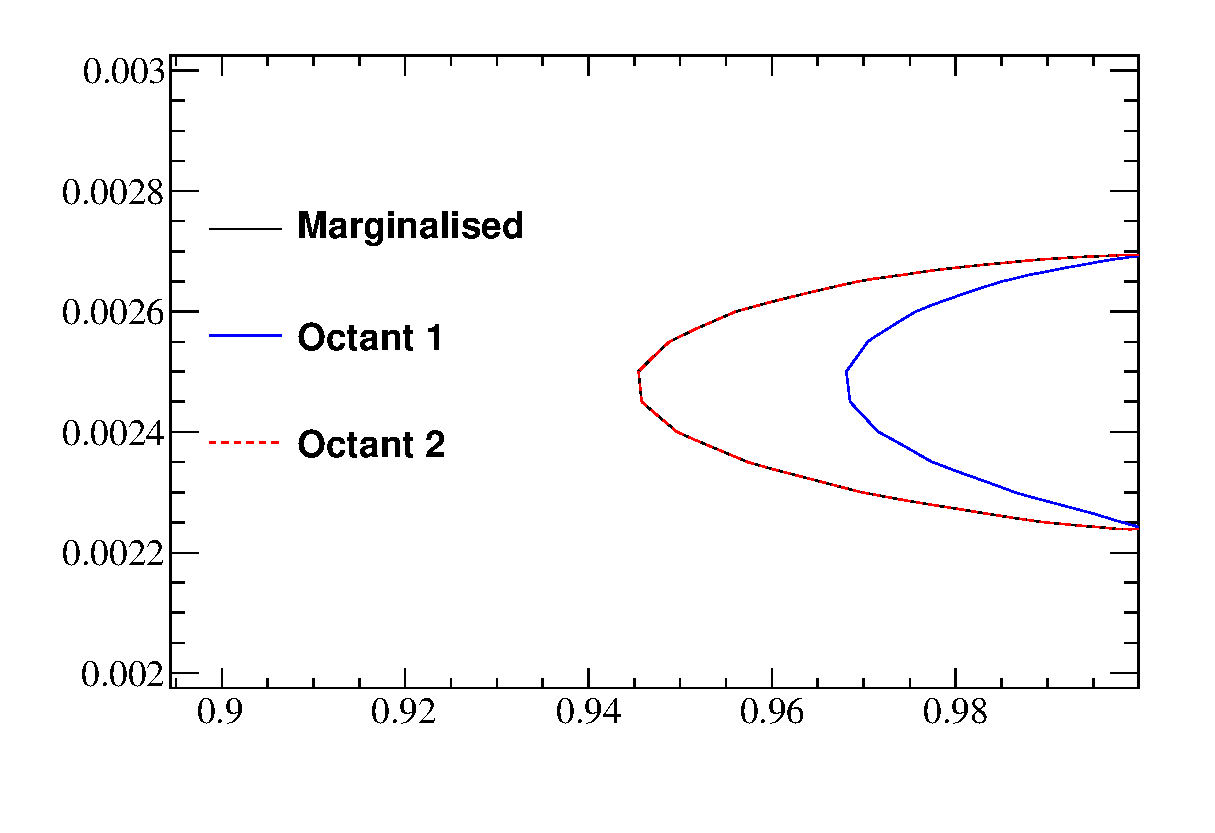
\includegraphics[width=30pc]{./images/sinsq2theta_conversion}
    \caption {
      68\% CL and 90\% CL allowed region (including systematics), 
      constructed with the constant-$\Delta\chi^{2}$ method,
      for the fit to the Run 1+2+3+4a dataset.
      The contour is converted into $\sin^2(2\theta_{23})$ in three ways:
      profiling over octant;
      assuming the first octant;
      assuming the second octant.
      The normal mass hierarchy is assumed.
    }
    \label{fig:contours_sinsq2theta_method}
  \end{figure*}
  


  % ........................................................................................................

\end{enumerate}


\subsection{
  Replies to comments received from Okumura-san - Aug 14, 2013 }

\begin{enumerate}

  % ........................................................................................................
  \vspace{5 mm}
\item
  {\em
    P10 Line 435:\\
    It is written that the uncertainty of $\theta_{13}$ is implemented in the fit by systematic parameter,
    and the uncertainty of $\delta_{CP}$ is included by throwing it randomly in the calculation of $\Delta \chi^2$ critical surface.
    I think that these different implementations may cause the cancellation of these systematic effect each other.
    As you know, both $\theta_{13}$ and $\delta_{CP}$ parameters can increase/decrease $\nu_\mu \rightarrow \nu_e$ oscillation.
    In the fitting procedure of toy-MC for critical $\chi^2$ value, assume that a toy MC is generated with
    a $\delta_{CP}$ value to enlarge $\nu_\mu \rightarrow \nu_e$ oscillation, then $\theta_{13}$ parameter should be moved so as to increase
    $\nu_\mu \rightarrow \nu_e$ oscillation to fit this toy MC distribution. And vice versa. As a result, some correlation is
    made between $\theta_{13}$ and $\delta_{CP}$, and systematic effect of $\delta_{CP}$ becomes under-estimated than expected I guess.
    Could you check for example, the correlation between generated $\delta_{CP}$ and fitted $\theta_{23}$ value?
  }\\
  \\
  No correlation has been found. See, for example,
  the correlation between generated $\delta_{CP}$ and fitted $\sin^2\theta_{23}$ residual
  in Fig.\ \ref{fig:dcp_sintheta23_correlation},
  and the correlation between generated $\delta_{CP}$ and fitted $|\Delta m^2_{32}|$ residual
  in Fig.\ \ref{fig:dcp_dm32sq_correlation} of this document.

  In v3 of the note, we will fit for $\delta_{CP}$ (see reply to Scott's comment 6).

  \begin{figure*}[htb]
    \begin{minipage}[t]{0.48\linewidth}
      \center
      \includegraphics[width=20pc]{{./images/dcp_sintheta23_correlation_0.37}.eps}
      \caption {
        Correlation between the input $\delta_{CP}$ value and the fitted
        $\sin^2\theta_{23}$ residual,
        computed from 5.1k toy MC experiments at $6.3933\times10^{20}$ POT,
        generated at
        at $\sin^2\theta_{23} = 0.37$ and $|\Delta m^2_{32}| = 2.4\times10^{−3}$ eV$^2$/c$^4$, including
        statistical fluctuations and with randomized systematic parameters.
      }
      \label{fig:dcp_sintheta23_correlation}
    \end{minipage}
    \hspace{0.06\linewidth}
    \begin{minipage}[t]{0.48\linewidth}
      \center
      \includegraphics[width=20pc]{{./images/dcp_dm32sq_correlation_0.37}.eps}
      \caption {
        Correlation between the input $\delta_{CP}$ value and the fitted
        $|\Delta m^2_{32}|$ residual,
        computed from 5.1k toy MC experiments at $6.3933\times10^{20}$ POT,
        generated at
        at $\sin^2\theta_{23} = 0.37$ and $|\Delta m^2_{32}| = 2.4\times10^{−3}$ eV$^2$/c$^4$, including
        statistical fluctuations and with randomized systematic parameters.
      }
      \label{fig:dcp_dm32sq_correlation}
    \end{minipage}
  \end{figure*}
  

  % ........................................................................................................

  \vspace{5 mm}
\item
  {\em
    P18 Table 3:\\
    It is written that you take the uncertainty of $\sin^2(\theta_{13})$ from PDG.
    But our T2K $\nu_e$ result using same RUN1-4 dataset gives larger $\theta_{13}$ best-fit value,
    and it is out of the uncertainty range you set. Since this analysis use same dataset as $\nu_e$,
    I'm not sure that this assumption is okay or not.
    I'm not sure that our best fit value of $\theta_{13}$ is due to effect of $\delta_{CP}$ or $\theta_{23}$,
    but we obtained this large $\theta_{13}$ with the assumption of $\delta_{CP}$=0 and $\sin^2(\theta_{23})=0.5$.
    In your $\nu_\mu$ analysis, this condition is similar I think; you apply fit with $\delta_{CP}$=0.
    Since we measured $\nu_\mu \rightarrow \nu_e$ oscillation more than expected by PDG value in the same dataset,
    isn't it better to take $\theta_{13}$ uncertainty in a consistent way with our $\nu_e$ result ?
    According to Figure 14, the uncertainty of $\theta_{13}$ is seen around oscillation peak,
    I guess it affect to $\sin^2(\theta_{23})$ uncertainty and it may be under-estimated.
  }\\
  \\
  In v3 of the note, we plan to fit for $\delta_{CP}$ (see reply to Scott's comment 6).
  Therefore we feel that using the reactor data is the natural choice,
  as this allows us to use a single number for the constraint term of $\sin^2\theta_{13}$ -
  if we used the T2K result we would need a multi-dimensional likelihood function
  to evaluate the correct $\sin^2\theta_{13}$ error for the penalty at the current value of
  $\sin^2\theta_{23}$ and $\delta_{CP}$.
  Using reactor data also prevents any correlations between $\nu_e$ and $\nu_\mu$ T2K
  data effecting the result.
  
  % ........................................................................................................

  \vspace{5 mm}
\item
  {\em
    P26 Table 7:\\
    You showed $\delta N_{sk}$/$N_{sk}$ for both BANFF prefit and postfit.
    I understand that errors related to BANFF parameters are reduced for postfit,
    but I don't understand that other errors are reduced largely. for example, that of
    $f_{\pi-less\Delta; t, r}$ changed from 6.3 to 4.9, $f_{NC1\pi^\pm; t}$ changed from 1.1 to 0.78.  Could you explain why ?
  }\\
  \\
  This is due to the fact that the BANFF fit changes the nominal spectrum, in addition to the size of the errors.
  Taking the example of $f_{NC1\pi^\pm; t}$,
  in the prefit case, the contribution to the total $N_{SK}$ from $NC1\pi^\pm$ modes is 3.21\%,%3.211806\%,
  and 40\% of this (the 1$\sigma$ $f_{NC1\pi^\pm; t}$ error) is 1.28\%.
  In the postfit case, the contribution to the total $N_{SK}$ from $NC1\pi^\pm$ modes is 2.60\%,%2.595826\%,
  and 40\% of this is 0.78\%.

  It is difficult to present a simple argument to confirm that $f_{\pi-less\Delta; t, r}$ is behaving correctly
  since it has both an $E_{reco}$ and $E_{true}$ dependence.
  % Contrib from modes PRE:                                      1pi :       41.235711 events ( 32.265295 \%)
  % Contrib from modes POST:                                     1pi :       36.017760 events ( 30.581505 \%)

  It should be noted that the prefit column of Tab.\ 10 of TN141
  is a direct copy of the postfit column, for all but the BANFF parameters.

  % ........................................................................................................

  \vspace{5 mm}
\item
  {\em
    P26 Table 7:\\
    You estimate $N_{sk}$ error due to $\delta_{CP}$ in this table. Could you explain how you estimate?
    You throw many toy MC with random $\delta_{CP}$, make $N_{sk}$ distribution, and take 1 sigma width of it? 
    Did you use this value in somewhere of your analysis program?
  }\\
  \\
  For the table in v1, the value is the maximum deviation of $\pm\pi/2$ tweaks.
  We agree that this is not the best thing to do for this parameter,
  therefore in v2 it is the 1 $\sigma$ width of 10000 uniform throws between $-\pi$ and $+\pi$.
  
  Note that for other parameters, the values were taken from the maximum deviation of $\pm1\sigma$ tweaks.
  This has been updated in v2 for parameters using splines, and oscillation parameters
  (parameters which are not pure normalisations)
  to use the same throw-based method.
  This was the same method that was used in Tab.\ 10 of TN141.
  
  % ........................................................................................................

  \vspace{5 mm}
\item
  {\em
    P39 Figure 45 \& 46:\\
    Can you compare these to those of previous analysis (TN-148)?
    I noticed that $f_{E; r}^{SK}$ pull deviates from zero this time while it was close to zero previously. Can you explain why?
  }\\
  \\
  A full comparison is not possible, since the SuperK detector efficiency \& FSI+SI parameters were separate in
  TN141.
  A comparison of SK energy scale, BANFF, and uncorrelated cross section parameters is shown in
  Fig.\ \ref{fig:compare_pulls} of this document, for 3 fits to the Run 1-3 data:
  \begin{itemize}
  \item TN141 method, 2012 SK data analysis;
  \item TN155 method, 2012 SK data analysis;
  \item TN155 method, 2013 SK data analysis.
  \end{itemize}
  The difference between 2012 and 2013 SK data analysis is described in
  TN148; for 1-ring $\mu$-like events, the effect is a spectrum change,
  two additional event accepted and one additional event rejected in 2013.
  All results assume normal mass hierarchy.
  
  The figure shows that differences in the pull distributions is due to a combination of
  two sources: 
  the differences betweens the TN141 \& TN155 fitters;
  and the difference in the SK energy spectrum for Run 1-3.

  We also refer you to the answer to Scott's question 9 - the error from the fit produced for $f_{E; r}^{SK}$
  is not as accurate as for the other parameters.
  
  \begin{figure*}[htb]
    \center
    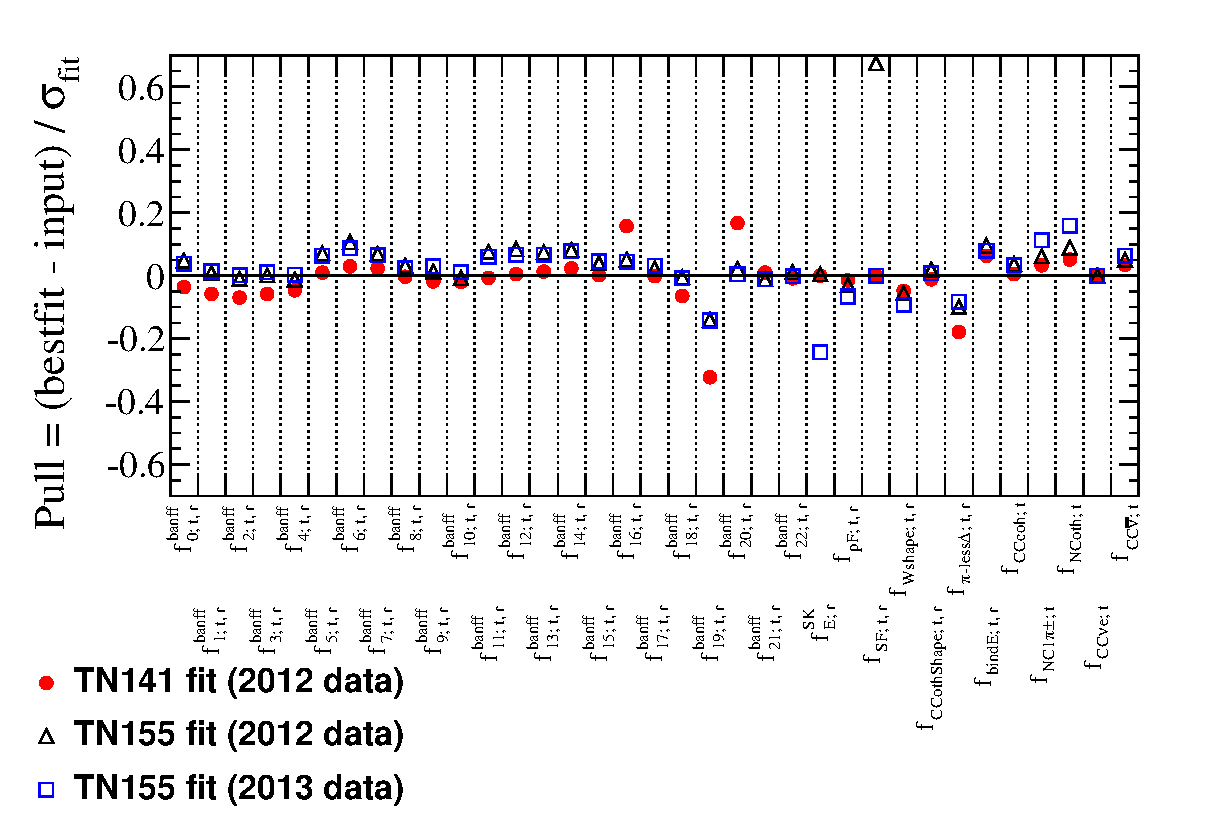
\includegraphics[width=30pc]{./images/pulls_comparison}
    \caption {
      Systematic parameter pulls for the fits to the Run 1+2+3 dataset.
      Results using the method of TN141 (2012 SK data analysis) and TN155 (2012 \& 2013 SK data analyses) are shown.
      The normal mass hierarchy is assumed.
    }
    \label{fig:compare_pulls}
  \end{figure*}


  % ........................................................................................................

  \vspace{5 mm}
\item
  {\em
    P57 Figure 69:\\
    You compared contours for const-$\Delta\chi^2$ and FC method. In page 10 Line 435, you described
    "the effect of $\delta_{CP}$ is handled by throwing ...."  Then I understand that the uncertainty
    due to $\delta_{CP}$ is included only in contour by FC method.
    Though it is not easy to compare in Fig 69 due to that FC analysis is not completed, it seems that
    there is not large difference between two contours due to $\delta_{CP}$. Is the effect of $\delta_{CP}$
    negligibly small ? Is it possible to quantify the effect of $\delta_{CP}$ ?
  }\\
  \\
  Please see the reply to Scott's comment 6.
  

  % ........................................................................................................



\end{enumerate}


\subsection{
  Replies to comments received from Antonio Ereditato, Ciro Pistillo and Martin Hierholzer - Aug 16, 2013 }

\begin{enumerate}

  % ........................................................................................................
  \vspace{5 mm}
\item
  {\em
    We support the proposal to extend the analyses to the full available data set (full 2013 statistics)
  }\\
  \\
  Please see the reply to Scott's comment 5.

  % ........................................................................................................
  \vspace{5 mm}
\item
  {\em
    We find that the approach used in TN164 where the old note (black text) is integrated with new (blue text)
    makes the whole more readable than having only the changes/additions listed.
  }\\
  \\
  We will take this into consideration when preparing technical notes in the future.

  % ........................................................................................................

\end{enumerate}


\subsection{
  Replies to comments received from Thomas Kutter - Aug 20, 2013 }

\begin{enumerate}

  % ........................................................................................................
  \vspace{5 mm}
\item
  {\em
    Page 9, l.371\\
    FGD 1 only, I assume ?
  }\\
  \\
  Correct, this has been updated.

  % ........................................................................................................
  \vspace{5 mm}
\item
  {\em
    Page 10, l.414 and all future occurrences:\\
    single mu-like ring $\rightarrow$ mu-like single ring OR single ring mu-like event  
  }\\
  \\
  Changed to 'single-ring $\mu$-like', as in page 6 of T2K-TN-034. 
  
  % ........................................................................................................
  \vspace{5 mm}
\item
  {\em
    Page 10, l. 426:\\
    - energy scale is 2.3\% in TN 164 $\rightarrow$ please provide and check your reference
  }\\
  \\
  The number 2.4\% comes from Sec.\ 7.2 of T2K-TN-148.
  The reference has been added.
  
  % ........................................................................................................
  \vspace{5 mm}
\item
  {\em
    Page 10, l.437:\\
    How were intranuclear and secondary interaction parameters and uncorrelated cross section parameters split
    into these classifications in the first place ? 
    Now they are being combined into single co-variance matrix. Please add some explanation to motivate this change.
  }\\
  \\
  The uncorrelated cross section errors were given to us by the NIWG.
  Please see TN108 and TN113 for details.

  The SuperK detector error efficiency matrix was given to us by T2KSK.
  Please see TN159 for details.

  The errors on parameters used to generate the FSI+SI matrix were provided by the NIWG.
  Please see TN108 and TN113 for details.
  The form of the FSI+SI matrix was chosen by oscillation analysers
  (both the VaLOR and (as then called) KIT groups)
  during the preparation for the Run 1-3 result,
  so as to have not too many nuisance parameters.
  Please see \url{http://www.t2k.org/asg/fluxmeasure/banffoa091312/numudisapp/view} for details
  of different binning schemes we tried\footnote{
    The 'fine' binning scheme was never completed;
    a covariance matrix for many bins could not be found.
  }.
  The conclusion is that we are not underestimating the error from FSI+SI with the matrix in this 6-bin form.

  The SuperK detector efficiency and FSI+SI matrices have been combined to reduce the number of nuisance parameters
  in the fit, and hence decrease the fit time.
  This is possible, because both the SuperK detector error matrix\footnote{
    TN141 used 3 $E_{reco}$ bins for $\nu_\mu+\bar{\nu_\mu}$ CCQE ring counting efficiency,
    and 1 bin for $\nu_\mu+\bar{\nu_\mu}$ CCQE other efficiencies.
    The 4 'other' and 'ring counting' parameters are combined into 3 parameters,
    giving a 6-parameter SuperK detector efficiency matrix.
  }, and the FSI+SI matrix are binned
  in the same way
  (3 $E_{reco}$ bins for $\nu_\mu+\bar{\nu_\mu}$ CCQE, 1 bin for $\nu_\mu+\bar{\nu_\mu}$ CCNQE,
  1 bin for $\nu_e+\bar{\nu_e}$ CC, 1 bin for NC).
  Fitting the combined matrix is mathematically equivalent to fitting the two matrices independently.
  
  % ........................................................................................................
  \vspace{5 mm}
\item
  {\em
    Page 11, l.442:  (related to Page 10. l. 422 and 424)\\
    was earlier mentioned to now be 6 parameter covariance matrix
    
    It would be good to add a short motivation or expected effect due to this change even in this document.
    As written it is not clear what was actually gained by introducing this.

    Presumably the details will be in TN 159 ?! 
  }\\
  \\
  The 7 parameters referred to in the bullet point are the 1 SuperK energy scale systematic,
  and the 6 parameter SuperK detector efficiency + FSI + SI error matrix.
  The bullet point list \& Tab.\ 1 headings have been updated.

  A sentence has been added to Sec.\ 2.3 to motivate the 7+6 $\rightarrow$ 6 parameter change.

  % ........................................................................................................
  \vspace{5 mm}
\item
  {\em
    Page 14:\\ die $\rightarrow$ due
  }\\
  \\
  Fixed
  
  % ........................................................................................................
  \vspace{5 mm}
\item
  {\em
    Page 14:\\
    $f_{CC\bar{\nu}; t}$  $\rightarrow$ please add reference for the 40\% uncertainty
  }\\
  \\
  This question initiated some email discussion between us and the NIWG convenoors. The summary is:

  \begin{itemize}
  \item The 40\% number came from either
    the most extreme excursions we found with NUANCE variations,
    or from the idea that there were $\sim$20\% discrepancies in neutrino
    CCQE data and theory, and that we weren't sure if those discrepancies would exist, flip sign and/or double, in anti-neutrinos.
  \item This was not included in a technical note.
  \item Since the time 40\% was agreed on (Oct 2012), MiniBooNE and MINERvA have published CCQE results for anti-neutrinos that,
    when compared to neutrino results, make it pretty clear that this 40\% is an overestimate.
    Something closer to 20\% for neutrino and anti-neutrino differences is sufficiently conservative.
  \end{itemize}

  In v3 of the note, we will use the 20\% number.
  
  % ........................................................................................................
  \vspace{5 mm}
\item
  {\em
    Page 18:\\
    why was $\delta_{CP}$ chosen to be zero ?
    
    $\rightarrow$ It would be good to add short explanation for choice of value.
    (e.g. "This is what others do." is not a good explanation.)
  }\\
  \\
  Since $\delta_{CP}$ has not been measured by any experiment, a well motivated choice of value to use
  is impossible.
  The constant-$\Delta\chi^2$ normal hierarchy contours for
  $\delta_{CP} = -\pi/2$, 0, $+\pi/2$, $+\pi$
  is shown
  in Fig.\ \ref{fig:constdchisqcontours_changedcp} of this document.
  It can be seen that changing $\delta_{CP}$ has almost no effect on the contour,
  therefore we feel that our choice of $\delta_{CP} = 0$ was sufficient.

  In v3 of the note, we will fit for $\delta_{CP}$.

  % ........................................................................................................
  \vspace{5 mm}
\item
  {\em
    Page 29:\\
    What causes the center peak to disappear with high statistics ?
    Or rather, what causes the center peak at lower statistics ?
  }\\
  \\
  This is a matter of statistical error.
  In Fig.\ 15, with low statistics, it is possible for the input to be such
  that there is more disappearance than the model allows, hence there
  is a build up of events at the point of maximal disappearance.
  In Fig.\ 16, with high statistics, the error is reduced such that
  the MC toys do not fluctuate enough to exhibit this behaviour.
  
  % ........................................................................................................
  \vspace{5 mm}
\item
  {\em
    Page 32, fig. 27, left most panel second row (and similar in other figures):\\
    Why is this distribution so much narrower ?
  }\\
  \\
  This the parameter is the spectral function.
  In toy experiment creation, it is thrown uniformly between 0 and 1.
  In fits, it is bound between 0 and 1\footnote{
    In v1 of the note, there was a Gaussian constraint applied to this parameter.
    In v3 of the note, we will turn off this constraint.
  }.
  Therefore it is not expected to have the same Gaussian distribution as the other parameters.
  
  % ........................................................................................................
  \vspace{5 mm}
\item
  {\em
    Page 38, Line 671:\\
    remove 4a
  }\\
  \\
  The figure caption was incorrect (Figs.\ 55 \& 56 are Run 1+2+3+4a data fits).
  The caption has been corrected.
  
  % ........................................................................................................
  \vspace{5 mm}
\item
  {\em
    Page 51, Figure 61 $\rightarrow$ Table XX :\\
    This should be table not figure
  }\\
  \\
  Fixed.
  
  % ........................................................................................................
  \vspace{5 mm}
\item
  {\em
    Page 54, fig. 65/66: \\
    "Efficiency holes" seem to be different for different values of $\Delta m^2$ / $\sin^2 \theta$ 
    This makes the plots confusing. Please add better description or unify holes.
  }\\
  \\
  Caption has been clarified.
  
  % ........................................................................................................
  \vspace{5 mm}
\item
  {\em
    Page 54, fig. 66: \\
    How many values of $\Delta m^2$ were considered to generate these plots ?
  }\\
  \\
  Figs.\ 65 \& 66 are an alternative way to represent the information in Fig.\ 64.
  A maximum of 6 values of $\Delta m^2$ were used.
  
  % ........................................................................................................
  \vspace{5 mm}
\item
  {\em
    Page 57, fig. 69:\\
    If I understand correctly const $\Delta \chi^2$ has $\delta_{CP}=0$ and whereas for FC method delta is randomized between $-\pi$ and $+\pi$.
    Please clarify whether the 3 flavor oscillation formula approximation from footnote on p.29 was used or whether delta dependent
    terms have been included. I assume the latter but please confirm.

    How do the const. $\Delta \chi^2$ contours change as function of delta ? 
    And why was delta =0 chosen ?  
  }\\
  \\
  All terms (including matter effects) are included in the oscillation probabilities.
  The purpose of the footnote is to show where the point of maximum disappearance approximately is,
  and it's dependce on the value of $\sin^2\theta_{13}$.

  Since $\delta_{CP}$ has not been measured by any experiment, a well motivated choice of value to use
  is impossible.
  The constant-$\Delta\chi^2$ normal hierarchy contours for
  $\delta_{CP} = -\pi/2$, 0, $+\pi/2$, $+\pi$
  is shown
  in Fig.\ \ref{fig:constdchisqcontours_changedcp} of this document.
  It can be seen that changing $\delta_{CP}$ has almost no effect on the contour,
  therefore we feel that our choice of $\delta_{CP} = 0$ is sufficient.

  In v3 of the note, we will fit for $\delta_{CP}$.

  
  % ........................................................................................................
  \vspace{5 mm}
\item
  {\em
    Page 57, fig. 70:\\
    It would be better to compare run 1-3 results and run 1-4 results more directly by using same treatment of octant.
  }\\
  \\
  We feel the best way to present comparisons is in terms of $\sin^2\theta_{23}$, and this plot
  has been added in v2 of the note.
  
  Fig.\ \ref{fig:contours_sinsq2theta_method} of this document shows the run 1-4a normal hierarchy contour converted into $\sin^2(2\theta_{23})$ in 3 ways:
  \begin{itemize}
  \item profiling over the octant, as in Fig.\ 70;
  \item assuming the first octant;
  \item assuming the second octant.
  \end{itemize}
  It can be seen that profiling is equivalent to the second octant assumption.

  Fig.\ \ref{fig:contours_sinsq2theta_external} of this document is a version of Fig.\ 70 with the two octant assumptions
  for the constant-$\Delta\chi^2$ method only.

  \begin{figure*}[htb]
    \center
    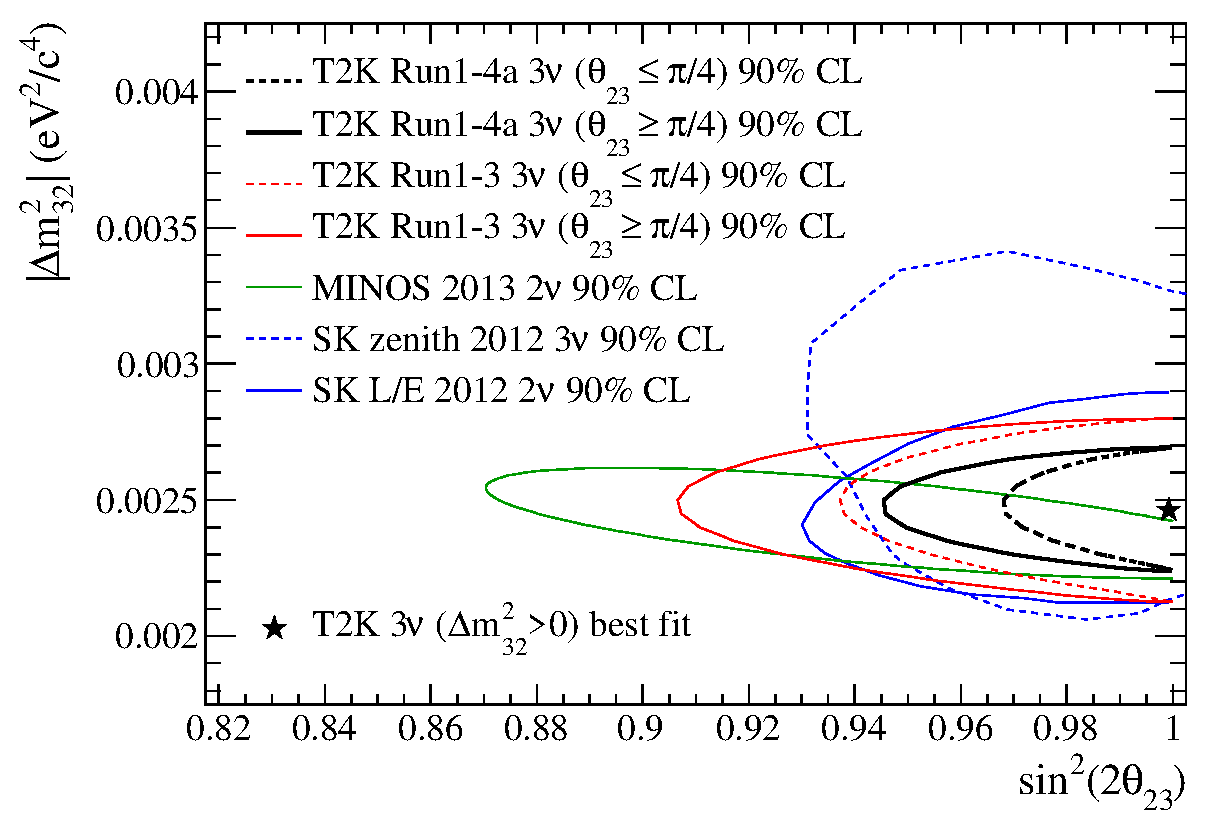
\includegraphics[width=30pc]{./images/contour_compare_constdchisqoctants_external_sinsq2theta23}
    \caption {
      Comparison between 90\% CL allowed regions 
      from MINOS, SuperK atmospherics, T2K Run 1+2+3,
      and the 90\% CL regions obtained from the VaLOR fit to the Run 1+2+3+4a dataset.
      Contours are obtained using the constant-$\Delta\chi^2$ method, and contours for both octant assumptions are shown.
      The normal mass hierarchy is assumed for all results.
    }
    \label{fig:contours_sinsq2theta_external}
  \end{figure*}


  %........................................................................................................

\end{enumerate}






 


 


 


 


 


 

 




\clearpage

\section{Summary of changes included in version 2 of T2K-TN-155 (released on Oct. 16, 2013)}

This section is designed to allow readers to keep track of the changes between versions of T2K-TN-155.
Table, figure, equation, footnote or citation numbers shown in black refer to version of 1,
{\color{red}whereas the numbers shown in red refer to version of 2}.
Both numbers are shown where possible.

\begin{itemize}

  %%%%%%% additions

\item Added motivation for combining SuperK detector efficiency and FSI+SI errors
  into a single matrix in Sec.\ 2.3 {\color{red}(2.3)}.

\item Clarified the number of SuperK parameters used in the fit in Sec. 3 {\color{red}(3)} and
  Tab.\ 1 {\color{red}(1)}.
  
\item Added footnote in Sec.\ 7.4 {\color{red}(7.4)} stating the critcal values of
  $\Delta\chi^2$ used in the constant-$\Delta\chi^2$ method.

\item Added an updated Feldman and Cousins $\Delta\chi^2_{critical}$ surface using
  finer binning in $\sin^2\theta_{23}$, and more stastics, to Figs.\ 64-66 {\color{red}(Figs.\ 63-65)}.
  The Feldman and Cousins contours in Figs.\ 67, 69 \& 70 {\color{red}(Figs.\ 66, 68 \& 70)}
  have also been updated.

\item Added a comparison between the T2K Run 1-4a contour and MINOS, SuperK atmospheric, and T2K Run 1-3 contours
  in terms of $\sin^2\theta_{23}$ in {Fig. 69}.
  
  %%%%%%% errors

\item Tab.\ 7 {\color{red}(7)} has been updated with a different method.
  In v1, the entries were the maximum deviation of $N_{SK}$ for $\pm1\sigma$ deviations.
  In v2, the entries for parameters which are not normalisations (parameters represented by splines,
  and oscillation parameters) 
  are the $1\sigma$ width from 10000 random throws.

\item Figs.\ 25-28, 33-36, 41-44 {\color{red}(25-28, 33-36, 41-44)} have been updated to contain
  more significant figures in the fit result parameters. This is to prevent fits which state
  that the sigma is $1\pm0.0$, even though they did not fail.

\item Figs.\ 59-61 {\color{red}(Figs.\ 59-60 \& Tab.\ 9)} have been updated with the correct one-parameter 90\% constant $\Delta \chi^2$ value
  of 2.71.
  
  %%%%%%% typos
  
\item Updated the referencing of the ND280 $\nu_\mu$ and BANFF analyses in the Secs.\ 1 \& 2 {\color{red}(1 \& 2)}, and
  Tab.\ 1 {\color{red}(1)}.

\item Added reference to the SuperK energy scale systematic in Sec.\ 2 {\color{red}(2)}.

\item Add units to Tab.\ 7 {\color{red}(7)}.

\item Corrected the caption of Figs.\ 55 \& 56 {\color{red}(55 \& 56)} to state that the spectra are for
  the Run 1+2+3+4a data fits.

\item Fig.\ 61 has been relabelled Tab.\ {\color{red}9}.

\item Clarified captions of Figs.\ 65 \& 66 {\color{red}(64 \& 65)} explaining why some points are missing.

\item Correctly state the name of the method (profiling, not marginalising) used to create the
  T2K contours in Fig.\ 70 {\color{red}(70)}.

\item Various typos have been fixed.
  
\end{itemize}







% References
%\input{numuosc2013a_review_references}

\end{document}

